\textbf{Java fournit la classe java.util.Hashtable comme implémentation de l’interface  java.util.Map. Pouvez-vous déterminer précisément de quelle variante de table de hachage il s’agit ? (Alexandre) }



La classe Hashtable du package java.util permet de créer des collections d'objets associés à des noms, en quelque sorte des dictionnaire. Une même Hashtable peut contenir des objets de classe quelconque.



\textbf{Java fournit-il d’autres implémentations de l’interface Map ? Faites un diagramme qui représente les interfaces et les classes qui se rapportent à Map et précisez ce qui, dans chaque cas, les caractérise.}

Oui, Java fournit d'autres implémentations de l'inferface Map

Les interfaces :
\begin{itemize}
	\item Bindings : Mapping des paires  clé/valeur, toutes les clés sont des strings
	\item ConcurrentMap<K,V> :  Ajoute les méthodes putIfAbsent, remove et replace par rapport à 
Map
	\item ConcurrentNavigableMap<K,V> : ConcurrentMap qui support les opérations sur les  NavigableMap
	\item  NavigableMap<K,V> : Ajoute des méthodes de navigation à Map
	\item SortedMap<K,V> : Les éléments sont comparables entre eux
\end{itemize}

Les classes :
\begin{itemize}
	\item AbstractMap :  Implémente quelques méthodes de java.util.Map. Tel que size() et 
isEmpty()
	\item Attributes : Map qui attribue un nom à un string
	\item AuthProvider :  Table de hashage avec login et mots de passe
	\item ConcurrentHashMap : Identique à Hashtable mais implémente en plus l'interface 
ConcurrentMap
	\item ConcurrentSkipListMap : Identique à Hashtable mais implémente en plus l'interface ConcurrentMap
	\item EnumMap : Ne prend comme key que des objets de la class Enum
	\item HashMap :  Équivalent à Hashtable mis à part qu'elle permet les éléments null 
	\item IdentityHashMap : Classe spéciale, elle n'implémente pas rigoureusement Map. C'est une table de hachage qui utilise == et non equals pour comparer deux éléments
	\item LinkedHashMap : Table de hachage avec une liste complémentaire reprenant les éléments dans l'ordre dans lequel ils ont été introduit
	\item Properties : Permet la lecture de fichier xml. Fait correspondre une valeur à une  propriété
	\item Provider :  Fait partie de java.security. Peut utiliser les algo DSA, SHA-1, MD5, RSA...
	\item RenderingHints :  Contient des éléments qui peuvent être utilisé par Graphics2D
	\item TabularDataSupport :  Implémente en plus de Map la classe TabularData
	\item TreeMap :  Implémente SortedMap, c'est un arbre ordonné
	\item UIDefaults : Fait pour les composant swing, contient les valeurs par défaut
	\item WeakHashMap : Même caractéristiques que HashMap. En plus retire les entrées dont la clé n'est plus utilisé de manière normal.
\end{itemize}

\begin{figure}[!h]
	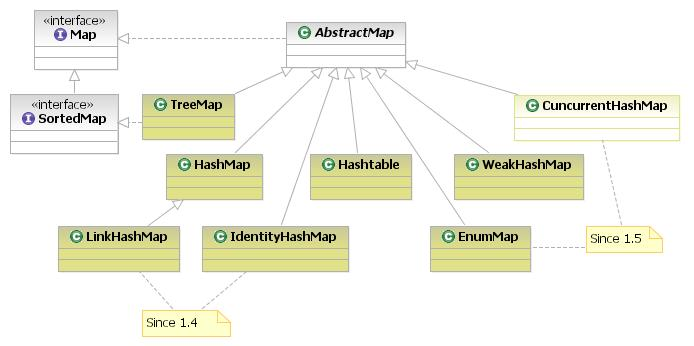
\includegraphics[height=7.5cm]{mapdia.jpg}
\end{figure}

\textbf{Qu’est-ce qui peut servir de clé pour une Hashtable en Java ? }
Tout objet non null peut être utilisé comme clé. Par exemple le nom d'un nombre peut-être utilisé comme clé.
\RestyleAlgo{boxed}
\begin{algorithm}
Hashtable<String, Integer> numbers
     = new Hashtable<String, Integer>()\;
   numbers.put("one", 1)\;
   numbers.put("two", 2)\;
   numbers.put("three", 3)\;
\end{algorithm}
